% Author	Rajath Shashidhara
% Email		rajath.shashidhara@gmail.com
%
% This work is licensed under the Creative Commons Attribution 4.0 International License. 
% To view a copy of this license, visit http://creativecommons.org/licenses/by/4.0/.

\chapter{AAH model driven by Circularly Polarized Light}
We consider a second model in the form of a perturbation by Circularly Polarized light. The electric field impacts both directions of the lattice periodically. However, as
stated in the previous chapter, this does not affect the definition of magnetic translation group. We can still define a magnetic unit cell and the magnetic Brillouin zone.

\section{Effective Hamiltonian}
This deriviation of Brillouin Wigner effective Hamiltonian is carried out in the same way as the previous model. Only results shall be stated here.
The k-space Hamiltonian is written as
\begin{equation}
 \begin{split} H(k_x, k_y, t)_{i,j} = 
                   \delta_{i+1,j} + \delta_{i,j+1} + 2 \lambda \cos(k_y - 2\pi\alpha\sin{\omega t} + 2\pi\alpha_0 j)\delta_{i,j} \\
                   + \delta_{i,1}\delta_{j,q} e^{-i(k_x -2\pi\alpha\cos{\omega t})q}+\delta_{i,q}\delta_{j,1} e^{i(k_x -2\pi\alpha\cos{\omega t})q}
                  \end{split}
\end{equation}
% The fourier components of the Hamiltonian are written in terms of fourier components of $\cos(r \cos(t)), \cos(r \sin(t)), \sin(r \cos(t)), \sin(r \sin(t))$.
% \begin{equation}
%  H_{i,j}^{m,n} = \begin{cases}
%                   
%                  \end{cases}
% \end{equation}
$H_{BW}$ is non-hermitian for this problem. This is an artifact of truncation of the $1/\omega$ series. The anti-hermitian part of the Hamiltonian can be ignored \cite{mikami2016brillouin}.
\section{Results}
The spectrum retains the Butterfly pattern. Any further analysis of the spectrum is not carried out.
\begin{figure}[h]
 \centering
 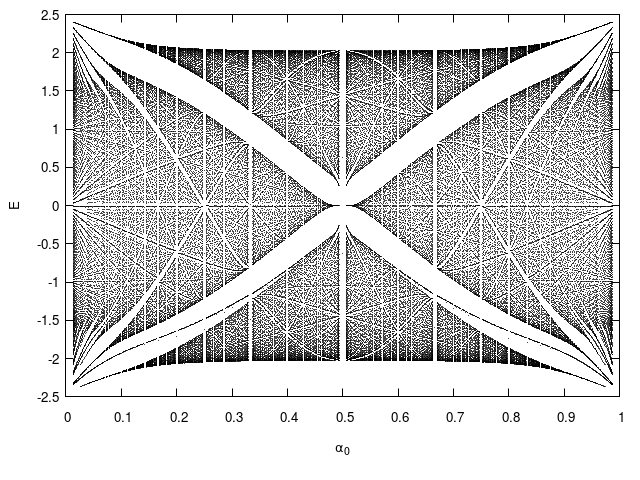
\includegraphics[width=0.7\textwidth]{cpl-spectrum}
 \caption{Plot of $E$ vs $\alpha_0$ for $\alpha=1$ and $\lambda=1$.}
\end{figure}

Chern numbers are also evaluated using the algorithm described in the previous chapter.
\begin{figure}[h]
 \centering
 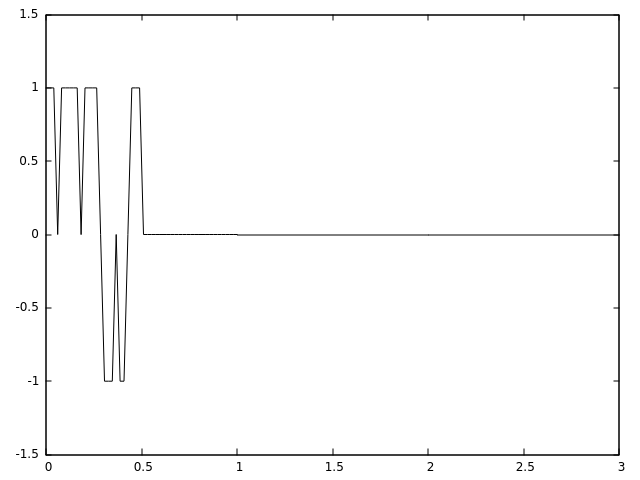
\includegraphics[width=0.45\textwidth]{chern-band1}\\
 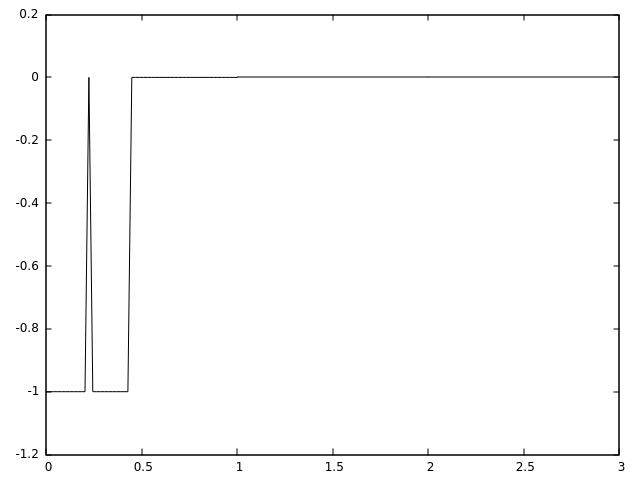
\includegraphics[width=0.45\textwidth]{chern-band2}
 \caption{Chern number vs $\alpha$ with $\alpha_0=1/3$ and $\lambda=1$ (a) Lowest energy band (b) Middle band.}
\end{figure}
\section{Discussion}
The chern numbers clearly undergo phase transitions. These topological phase transitions are seem to have no discernible pattern. One important observation is that after a critical value
of $\alpha$, all chern numbers go to zero.